\documentclass{article}

% if you need to pass options to natbib, use, e.g.:
% \PassOptionsToPackage{numbers, compress}{natbib}
% before loading nips_2016
%
% to avoid loading the natbib package, add option nonatbib:
% \usepackage[nonatbib]{nips_2016}

\usepackage[final]{nips_2016}

% to compile a camera-ready version, add the [final] option, e.g.:
% \usepackage[final]{nips_2016}

\usepackage[utf8]{inputenc} % allow utf-8 input
\usepackage[T1]{fontenc}    % use 8-bit T1 fonts
\usepackage{hyperref}       % hyperlinks
\usepackage{url}            % simple URL typesetting
\usepackage{booktabs}       % professional-quality tables
\usepackage{amsfonts}       % blackboard math symbols
\usepackage{nicefrac}       % compact symbols for 1/2, etc.
\usepackage{microtype}      % microtypography

\usepackage{amsmath,amssymb,amsthm,graphics,subfigure,graphicx,enumerate,bbm} 
\usepackage[table,xcdraw]{xcolor}
\usepackage{tikz}
\usepackage{tabularx,ctable,array}
\usepackage{natbib,caption}
\usepackage{algorithm,algpseudocode}
\usepackage{parnotes,float,multicol}
\usetikzlibrary{positioning}
\newcolumntype{?}{!{\vrule width 1pt}}
\newcommand{\R}{\mathbb{R}}
\newcommand{\C}{\mathbb{C}} 
\newcommand{\N}{\mathcal{N}} 
\newcommand{\T}{\mathcal{T}}
\newcommand{\M}{\tilde{M}}
\newcommand{\tmij}{\tilde{m}_{ij}}
\newcommand{\mij}{{m}_{ij}}
\newcommand{\mjk}{{m}_{jk}}
\newcommand{\boldc}{\boldsymbol c}
\newcommand{\boldd}{\boldsymbol d}
\newcommand{\boldm}{\boldsymbol m}
\newcommand{\boldvd}{\boldsymbol v_d}
\newcommand{\boldve}{\boldsymbol v_e}
\newcommand{\boldvc}{\boldsymbol v_{c'}}
\newcommand{\boldvci}{\boldsymbol v_{c_{<i}}}
\newcommand{\boldy}{\boldsymbol y}
\newcommand{\boldx}{\boldsymbol x}



\title{Chord2Vec - Learning Chords Embeddings}

% The \author macro works with any number of authors. There are two
% commands used to separate the names and addresses of multiple
% authors: \And and \AND.
%
% Using \And between authors leaves it to LaTeX to determine where to
% break the lines. Using \AND forces a line break at that point. So,
% if LaTeX puts 3 of 4 authors names on the first line, and the last
% on the second line, try using \AND instead of \And before the third
% author name.

\author{
   Coauthor1 \\
   Affiliation \\
   Address \\
   \texttt{email} \\
  %% examples of more authors
   \And
   Coauthor2 \\
   Affiliation \\
   Address \\
   \texttt{email} \\
   \AND
   Coauthor3 \\
   Affiliation \\
   Address \\
   \texttt{email} \\
  \And
   Coauthor \\
   Affiliation \\
   Address \\
   \texttt{email} \\
  %% \And
  %% Coauthor \\
  %% Affiliation \\
  %% Address \\
  %% \texttt{email} \\
}

\newcommand{\skipgram}{\textit{Skip-gram}}
\newcommand{\wordtovec}{\textit{word2vec}}
\newcommand{\seqtoseq}{\textit{sequence-to-sequence}}
\newcommand{\ie}{\textit{i.e.}}

\begin{document}
% \nipsfinalcopy is no longer used

\maketitle

\begin{abstract}
  In natural language processing, the well-known \skipgram\ model learns vector representations of words that carry meaningful syntactic and semantic information. In our work, we investigate whether similar high-quality embeddings can be found for symbolic music data. We introduce three NLP inspired models to learn vector representations of chords and we evaluate their performance. We show that an adaptation of the \seqtoseq\ model is by far superior to the other proposed model. 
  
\end{abstract}

\section{Introduction}

The \wordtovec\ model by \citet{mik2013} learns vector representations of words that carry syntactic and semantic information which has proven powerful in various natural language processing (NLP) tasks. In this work, we investigate whether similar embeddings can be found for symbolic music data. % As in language, arbitrary encodings of polyphonic music provide no useful information regarding the relationships that may exist between the individual musical chords. The main goal of this study is to introduce techniques that can be used for learning high-quality embedding chord vectors from sequences of polyphonic music. 

In the spirit of the \skipgram\ model \citep{mik2013}, the heuristic we use to achieve this involves finding chord representations that are useful for predicting the temporally neighboring chords in our corpus of musical pieces. Given such a corpus of ordered musical chords  $\T = \{\boldd_1, \boldd_2, \ldots, \boldd_T\}$ and a neighborhood of size $2j$ defined by $ C(\boldd_t) = \{\boldd_{t+j}, -m \leq j \leq m , j \neq 0\}$, the objective is to maximize the average log probability with respect to some model parameters~$\theta$:
%
\begin{equation}
\max_{\theta} \frac{1}{|\T|}\sum_{\boldd_t \in \T} \sum_{\boldc' \in C(\boldd_t)} \log p(\boldc = \boldc'|\boldd_t, \theta)
 \,,
\label{eq:c2v_obj}
\end{equation} 
%
where for the remainder of this report, we assume $j=1$.
Whereas text can be represented as a sequence of words, each encoded by a ``one-hot" vector, for music we need a ``many-hot" vector to represent a chord. This is because more than one note may sound simultaneously.

In the next \autoref{sec:models} we introduce our three NLP inspired models. The first is based on a simple conditional independence assumption, the second relaxes this assumption, while the third adopts a more sophisticated \seqtoseq\ architecture. In \autoref{sec:experiments} we evaluate the models on five datasets, before summarising and suggesting directions for future work in \autoref{sec:summary}. 

\section{The Proposed Models}
\label{sec:models}
\subsection{Bilinear model}
Our first model is a simplistic adaptation of the \skipgram\ model introduced by \citet{mik2013} to the many-hot case. Here, we replace the last softmax layer in \skipgram\ by a sigmoid layer with $N$ outputs, to predict each note individually.  

The architecture is a feed forward neural network consisting of input, hidden and output layers. At the input layer, a chord is encoded using a fixed length binary vector $\nolinebreak{\boldc = \{c_1, c_2, \ldots, c_N\}\in \{0,1\}^N}$, where $N$ is the number of notes in the vocabulary. In this chord representation, the entries that are set to $1$ correspond to the notes that are \textit{on} in the chord, whereas the notes that are \textit{off} are set to $0$. 

The weights between the input layer and the hidden layer can be represented by a matrix $M\in \R^{D \times N}$. Similarly, the weights between the hidden layer and the output layer can be represented by a matrix $\M\in \R^{N \times D}$. 

%\begin{figure}[ht]
%\centering 
%
%\tikzset{%
%   neuron missing/.style={
%    draw=none, 
%    scale=1.5,
%    text height=0.333cm,
%    execute at begin node=\color{black}$\vdots$
%  },
%}
%
%\begin{tikzpicture}[x=1.3cm, y=.80cm, >=stealth]
%
%\foreach \m [count=\y] in {1,2,3}
%  \node [circle,fill=gray!50,minimum size=0.5cm ] (input-\m) at (0,2.5-\y) {};
%  
%\foreach \m [count=\y] in {4}
%  \node [circle,fill=gray!50,minimum size=0.5cm ] (input-\m) at (0,-2.05) {};
%  
% \node [neuron missing]  at (0,-1.2) {};
%
%\foreach \m [count=\y] in {1}
%  \node [circle,fill=gray!50,minimum size=0.5cm ] (hidden-\m) at (2,0.75) {};
%  
%\foreach \m [count=\y] in {2}
%  \node [circle,fill=gray!50,minimum size=0.5cm ] (hidden-\m) at (2,-1.45) {};
%  
% \node [neuron missing]  at (2,-0.3) {};
%
%\foreach \m [count=\y] in {1,2,3}
%  \node [circle,fill=gray!50,minimum size=0.5cm ] (output-\m) at (4,2.5-\y) {};
%  
%\foreach \m [count=\y] in {4}
%  \node [circle,fill=gray!50,minimum size=0.5cm ] (output-\m) at (4,-2.05) {};
%  
% \node [neuron missing]  at (4,-1.2) {};
%
%\foreach \l [count=\i] in {1,2,3,N}
%  \draw [<-] (input-\i) -- ++(-1,0)
%    node [above, midway] {$d_{\l}$};
%
%\foreach \l [count=\i] in {1,D}
%  \node [above] at (hidden-\i.north) {$h_{\l}$};
%
%\foreach \l [count=\i] in {1,2,3,N}
%  \draw [->] (output-\i) -- ++(1,0)
%    node [above, midway] {$c_{ \l}$};
%
%\foreach \i in {1,...,4}
%  \foreach \j in {1,...,2}
%    \draw [->] (input-\i) -- (hidden-\j);
%
%\foreach \i in {1,...,2}
%  \foreach \j in {1,...,4}
%    \draw [->] (hidden-\i) -- (output-\j);
%
%\end{tikzpicture}
%\caption{Linear model architecture}
%\label{fig:lin-archi}
%\end{figure}

The $D$-dimensional vector representation $\boldvd$ of the associated chord $\boldd$ is simply the normalized sum of the columns of $M$ that correspond to the notes occurring in $\boldd \in \{0,1\}^N$:
\[ \boldvd = M\frac{ \boldd}{\| \boldd \|_1}
\]
To compute the probabilities in (\ref{eq:c2v_obj}) under this model, we make a  conditional independence assumption between the notes in a context chord $\boldc$ given a chord $\boldd$, \ie\
%
\begin{equation}
p(\boldc =\boldc' | \boldd) = \prod_{i=1}^N  p(c_i =c_i'|  \boldd) \,.
\end{equation} 
%
Using weights matrices $M$ and $\M$, we define a scoring function $\nobreak{h: \mathcal{N}~\times~\mathcal{C}\mapsto\mathbb{R}}$ by
\begin{equation}
h(i,\boldd) =  \M_{(:,i)} \boldvd \,,
\end{equation}
where $\M_{(:,i)}$ denotes the $i$'th row of $\M$. We then model the required conditional probabilities as
% \begin{equation}
% p(c_i =c_i'|  \boldd) = \left\{
%                 \begin{array}{lll}
%                   \sigma\big( h(i,\boldd) \big) = \frac{\exp(h(i,\boldd))}{1 + \exp(h(i,\boldd))} & c_i' = 1 \\
%                   1- \sigma\big( h(i,\boldd) \big) = \sigma\big( - h(i,\boldd) \big) = \frac{1}{1 + \exp(h(i,\boldd))} & c_i' = 0\\
%                 \end{array}
%               \right.
% \end{equation}
\begin{equation}
p(c_i =1|\boldd) = \sigma\big( h(i,\boldd) \big),
\end{equation}
where $\sigma(x)=1/(1+\exp(-x))$ is the usual sigmoid function.
This model is not expected to perform well, mainly because of the independence assumption between the notes in a chord. In fact, it is very likely that there is a strong dependency between the notes appearing in a chord. In the next section, we introduce a model that does not make such an independence assumption. 

\subsection{Autoregressive model}

To overcome the necessity of making the independence assumption between the notes appearing in a chord while retaining tractability, we introduce another model inspired by the The Neural Autoregressive Distribution Estimator (NADE) which models the distribution of high-dimensional vectors of discrete variables \citep{larochelle2011}. We decompose the context chord probability distribution according to the chain rule, so that
%
\begin{equation}
p(\boldc =\boldc' | \boldd) = \prod_{i=1}^N  p(c_i =c_i'|  \boldd, c_{<i}) \,,
\end{equation} 
%
where $c_{<i} = \{c_1, \ldots, c_{i-1}\}$. We define a new scoring function
%
\begin{equation}
h(i,\boldd,c_{<i}) =  W_{:,i} \cdot (\boldvd + \boldvci) \,,
\end{equation}
%
where $M, L \in \R^{D \times N}$ and $W\in \R^{N \times D}$ are weight matrices, $\boldvci=\sum_{j<i}  L_{:,j} c_j$ and $\boldvd = M\frac{ \boldd}{\| \boldd \|_1}$ is the D-dimensional vector representation of our chord.
As before we let
%
% \begin{equation}
% p(c_i =c_i'|  \boldd, c_{<i}) = \left\{
%                 \begin{array}{lll}
%                   \sigma\big( W_{:,i} \cdot (\boldvd + \boldvci) \big)  & c_i' = 1 \\
%                   1- \sigma\big( W_{:,i} \cdot (\boldvd + \boldvci) \big)  & c_i' = 0\\
%                 \end{array}
%               \right.
% \end{equation}
\begin{equation}
p(c_i =1|\boldd) = \sigma\big( h(i,\boldd,c_{<i}) \big).
\end{equation}
Hence, like NADE we retain tractability while relaxing the conditional independence assumption.
%
\subsection{Sequence-to-sequence model}
%
Finally, we propose to adapt the famous \seqtoseq\ model \citep{SutskeverVL14} to the task of learning chord embeddings. In language models, RNNs are useful for predicting future elements of a sequence given prior elements. The \seqtoseq\ model builds on top of language models  to create translation models that operate on two sequences -- the input sequence and the translated output sequence. It looks at each element of the sequence and tries to sequentially predict the next elements of the output sequence. We then suggest to train a \seqtoseq\ model to predict the elements in the temporally neighboring chords given an input chords.    
In this setting, a chord $c$ is represented as an (arbitrary length) ordered sequence of notes, so that $c_i\leq c_{i+1}\in\left\{1,2,\dots,N\right\}$.

Appropriately, \seqtoseq\ models learn a mapping of input sequences of varying lengths to output sequences also of varying lengths, using a neural network architecture known as an RNN Encoder-Decoder. 
%\begin{figure}[ht]
%\centering
%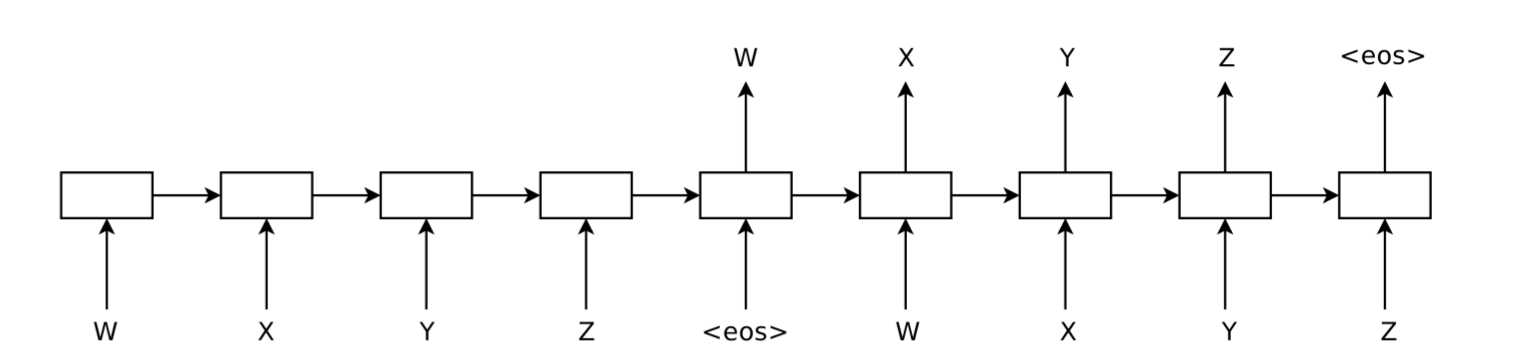
\includegraphics[width=1.0\linewidth]{figures/seq2seq.png}
%\caption{\label{fig:seq2seq}Sequence-to-sequence (\citet{SutskeverVL14})}
%\end{figure}
An LSTM encoder is used to map the input sequence to a fixed length vector, and another LSTM decoder is then used to extract the output sequence from this vector. The general goal is to estimate 
$
p(y_1,\ldots,y_{T'} | x_1, \ldots, x_T)\,,
$
where $x_1, \ldots, x_T$ and  $y_1,\ldots,y_{T'}$
are the input and output sequences, respectively. %, and $T'$ and $T$ need not to be equal. 
%
The objective is
%
\begin{equation}
\max_{\theta} \frac{1}{|\T|} \sum_{(\boldsymbol{x},\boldsymbol{y}) \in \T} \log p(\boldsymbol{y}|\boldsymbol{x},\theta) \,,
\label{eq:seq2seq_obj}
\end{equation}
%
where $\boldsymbol{y}$ is a correct output given the input $\boldsymbol{x}$, $\T$ is the training set and $\theta$ is the set of the model parameters. 
The encoder and decoder are jointly trained to maximize the objective according to $\theta$.

The model estimates the conditional probability $p(y_1,\ldots,y_{T'} | x_1, \ldots, x_T)$ by first obtaining the fixed-length vector representation $\boldsymbol{v}$ of the input sequence (given by the last state of the LSTM encoder) and then computing the probability of $y_1,\ldots,y_{T'} $ with the LSTM decoder: 
%
\begin{equation}
p(y_1,\ldots,y_{T'} | x_1, \ldots, x_T,\theta) = \prod_{t=1}^{T'} p(y_t|\boldsymbol{v}, y_1,\ldots,y_{t-1},\theta)
\end{equation}
%
% The sequence-to-sequence model can be used to learn embeddings for chords, by training the model to learn the context of a given chord. 
%
% At the chord level, the encoder projects all notes in a chord into a joint note representation and a decoder generates all notes in a chord given a chord representation and previously generated notes.
In our setting, we form the $\boldsymbol{y}$ by concatenating elements of the neighbourhood chords. We appropriately insert a special symbol (say, $\epsilon$) which serves as an end of chord marker (similar to an end of sentence marker in NLP). For example, if $\boldd=\boldc_i=(60,64,67)$ and the neighbourhood consists of chords $\boldc_{i-1}=(59)$ and $\boldc_{i+1}=(62,65,69)$, then we have $\boldx=(60,62,67)$ as our input sequence $\boldy=(59,\epsilon,62,65,69,\epsilon)$ as our output sequence. We take the corresponding $\boldsymbol{v}$ as the embedding for $\boldd$.
% indicating the end of the first chord. The goal then is to estimate
% $
% p(c_1, \ldots, c_T | d_1,\ldots,d_{T'})\,,
% $
% where  $d_1, \ldots, d_{T'}$ and $c_1, \ldots, c_T$ are in $\N$, $d = d_1, \ldots, d_{T'}$ is an input chord and $c_{t+j} =n^{(j)}_1, \ldots, n^{(j)}_T$ is a neighbor of $c$.
%
% If $C(d)$ denotes the set of chords that are in the neighborhood of the chord $d$, then the objective in (\ref{eq:seq2seq_obj}) can be written as:
%
% \begin{equation}
% \max_{\theta} \frac{1}{|\T|} \sum_{d \in \T} \sum_{c\in C(d)} \sum_{t=1}^{|c|} \log p(c_t | v_d, c_1, \ldots, c_{t-1})  \,,
% \label{eq:c2c_obj}
% \end{equation}
%
% where $v_d$ is the vector representation of the input chord $d$. 
%
\section{Experiments}
\label{sec:experiments}

%\subsection{Data sets}
We consider five datasets of varying complexity, taken from \cite{bl}:
\begin{itemize}
  \item \textbf{JSB Chorales}: 382 chorales by J.S. Bach with the split of  \citet{allan2005harmonising}.
 \item \textbf{Nottingham}: 1200 folk tunes with chords instantiated from the ABC format.
\item \textbf{MuseData}: electronic library of orchestral and piano classical music from CCARH.
\item \textbf{Piano-midi.de}: classical piano MIDI archive split according to \citet{poliner2007discriminative}
\item \textbf{Mix}: the union of all the above.
\end{itemize}
%\begin{itemize}
%\item[] \textbf{JSB Chorales}: corpus of 382 four-part harmonized chorales by J.S. Bach with the split of  \citet{allan2005harmonising}
%\item[] \textbf{Nottingham}: collection of 1200 folk tunes with chords instantiated from the ABC format
%\item[] \textbf{MuseData}: electronic library of orchestral and piano classical music from CCARH
%\item[] \textbf{Piano-midi.de}: classical piano MIDI archive split according to \citet{poliner2007discriminative}
%\item[] \textbf{Mix}: a collection of all above datasets.
%\end{itemize}
The polyphony varies from 0 to 15 and the average number of simultaneous notes is $3.9$. The range of notes spans the whole range of piano from A0 to C8, \ie\ $N = |\N| = 88$. We also augmented the training data as follows: we transpose each piece by $\phi$ semi-tones, for $\phi = -6, -5, \dots, 4, 5.$
%
\subsection{Baselines}
In addition to the previously mentioned models, we compare our results with the following models. \textbf{Random} is the simplest baseline with uniform $p(c_i = c_i' | d ) = 0.5$. \textbf{Marginal} is the smoothed empirical distribution of the notes in the training data, $p(c_i = 1 | d )= \frac{z_i + \alpha}{|\T|+\alpha}$ where $z_i$ is the number of the occurrences of note $i$ in the training set and $\alpha = 1$ is the smoothing constant.
%
\subsubsection{Implementation Details}
The linear chord2vec model and the autoregressive chord2vec were trained in batches of size 128 with  Adam Optimizer using $D = 1024$. Each model is optimized for 200 epochs, but the final model is the one leading to the lowest validation error.  
%
Our sequence-to-sequence model architecture is a multi-layer LSTM with 2 layers of 512 hidden units each. To allow sequences of varying length, standard bucketing and padding methods are used. We append to each target chord an end-of-sequence symbol.
%
We implemented all three models using Google's Tensorflow library.

\section{Results}

The negative log likelihoods on the test data for all models and on all data sets are presented in Table~\ref{tab:results}. First, we observe that our simple linear model, despite the independence assumptions, is able to actually learn something beyond the marginal distribution of the training set. Secondly, as expected, we observe that the autoregressive model achieves better scores than the simple linear model on all data sets, confirming our hypothesis that the notes in a chord are not independent of each other. Lastly, it appears that the Sequence-to-Sequence model is by far the strongest model overall.   
%
\begin{table}[ht]
\centering
\caption{Average negative log likelihood per chord for the test set.}
\begin{tabular}{l?lllll}
\hline
Model   & JSB Chorales & Nottingham & MuseData & Piano-midi.de & Mix \\ \hline
Random & 61.00 & 60.99 & 60.99 & 60.99 & 60.99\\ 
Marginal & 12.23 & 10.44 & 23.75 & 17.36 & 15.26 \\ 
Linear c2v & 9.77 & 5.76 & 15.41 &12.68 & 12.17  \\ 
Autoreg. c2v & 6.18 & 3.98 &14.49 & 10.18 & 7.42 \\ 
Seq2Seq c2v & 1.11 &  0.50 & 1.52 & 1.78 & 1.22 
\label{tab:results}
\end{tabular}
\end{table}
%
\section{Summary and Future work}
\label{sec:summary}
Our study has revealed that the Sequence-to-Sequence model is dramatically superior to our simpler methods. However, in the case of text classification problems, it has been shown that simpler architectures can lead to results that are comparable to deep learning models in terms of accuracy, but much faster for training and evaluation \citep{JoulinGBM16}.
With this in mind, a direction for future work would be to develop another model based on the \skipgram\ model but without making the assumption of independence between the notes occurring in a chord. 

One could also visualize the learned vectors by using dimensionality reduction techniques. An inspection of such low dimension vectors could help understanding whether the embedding vectors capture interesting musically relevant information.

Another interesting direction involves combining our \seqtoseq\ based chord embedding model with an additional temporal recurrence, in order to model entire pieces of music.

\bibliographystyle{plainnat}
\bibliography{bibli.bib} 

\end{document}
